\documentclass[a4paper,fleqn,review]{cas-sc}
\usepackage[authoryear,longnamesfirst]{natbib}
\usepackage[american]{babel}
\usepackage{amsmath, amssymb, geometry, graphicx, booktabs, multirow, makecell}
\usepackage{todonotes}
\usepackage{tcolorbox}
\usepackage{placeins}
\usepackage{caption}
\usepackage[hypcap=false]{caption}

\def\tsc#1{\csdef{#1}{\textsc{\lowercase{#1}}\xspace}}
\tsc{WGM}
\tsc{QE}
\tsc{EP}
\tsc{PMS}
\tsc{BEC}
\tsc{DE}

\tcbuselibrary{minted,breakable,xparse,skins}
\definecolor{bg}{gray}{0.95}
\DeclareTCBListing{mintedbox}{O{}m!O{}}{%
	breakable=true,
	before skip=10pt, 
	after skip=10pt,
	listing engine=minted,
	listing only,
	minted language=#2,
	minted style=default,
	minted options={%
		linenos,
		gobble=0,
		breaklines=true,
		breakafter=,,
		fontsize=\small,
		numbersep=8pt,
		#1},
	boxsep=0pt,
	left skip=0pt,
	right skip=0pt,
	left=20pt,
	right=0pt,
	top=3pt,
	bottom=3pt,
	arc=5pt,
	leftrule=0pt,
	rightrule=0pt,
	bottomrule=2pt,
	toprule=2pt,
	colback=bg,
	colframe=orange!70,
	enhanced,
	overlay={%
		\begin{tcbclipinterior}
			\fill[orange!20!white] (frame.south west) rectangle ([xshift=20pt]frame.north west);
	\end{tcbclipinterior}},
	#3}
\usepackage{csquotes}

\newcommand{\ldash}{--- }

\newtheorem{theorem}{Formula}
\newdefinition{definition}{Definition}
\newproof{pot}{Derivation Outline for Formula}

\renewcommand{\subsubsectionautorefname}{Formula}
\renewcommand{\subsectionautorefname}{Formula}
\renewcommand{\sectionautorefname}{Formula}


\begin{document}

%\begin{frontmatter}
\let\WriteBookmarks\relax
\def\floatpagepagefraction{1}
\def\textpagefraction{.001}
\shorttitle{Normalized Performance Measure}
\shortauthors{Kartikeya Mishra}


\title [mode = title]{A \textsf{Novel} Method for Ranking Group Performance}            
\tnotemark[1]

\tnotetext[1]{This research did not receive any specific grant from funding agencies in the public, commercial, or not-for-profit sectors.}          

\author[1]{Kartikeya Mishra}[type=editor,
auid=000,
orcid=0009-0001-3311-3955,
linkedin=ninjaadvisor]
\ead{kartik.maxwell@gmail.com}


\affiliation[1]{organization={Independent Researcher},
	addressline={50-D, Block E-3, Shatabdi Vihar, Sector 52}, 
	city={Noida},
	%               citysep={}, % Uncomment if no comma needed between city and postcode
	postcode={201307}, 
	state={Uttar Pradesh},
	country={India}}	

\credit{}

\begin{abstract}
	This paper introduces a novel non-parametric method for calculating group-level performance scores, incorporating rank sums, weight bias adjustments for unequal group sizes, and cross-collection interpretability. Theoretical derivations, mathematical and numerical validations with a detailed example are discussed.
\end{abstract}

%\begin{graphicalabstract}
%	\centering
%	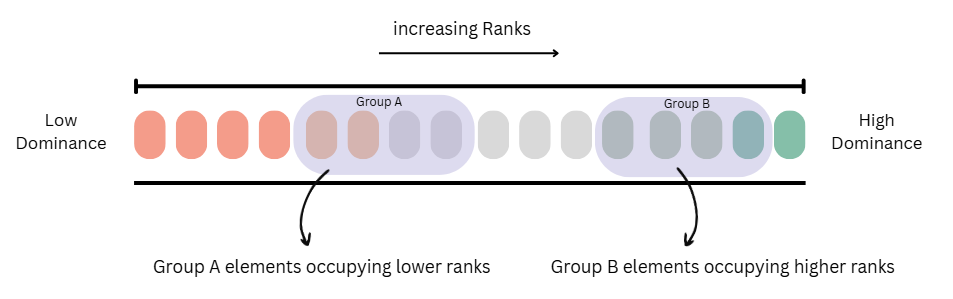
\includegraphics[scale=0.5]{dominance-intuition}
%\end{graphicalabstract}
%
%\begin{highlights}
%	\item Research highlights item 1
%	\item Research highlights item 2
%	\item Research highlights item 3
%\end{highlights}

\begin{keywords}
	Normalized Rank Comparison \sep Performance Analysis \sep Weighted Bias  \sep Statistical Methods
\end{keywords}
%\end{frontmatter}
\maketitle
\section{Introduction}
This formula can numerically identify the performance of a group $P_i$ within a collection of groups containing unequal number of elements. This novel approach takes into account weight bias inherent in the formula itself. The performance measure, $P_i$ numerically falls in the normalized range of [0,1] from worst to best performance on a universal scale, is interpretable and practical, thus can be visualized as 0 to 100\% prominence in performance via $P_i * 100$. 
This standardized scale can be used to compare within cross-collection with different scales. The \autoref{fig:superset-collection} illustrates towards which scenario, this formula can be applied to.
\begin{figure}
	\centering   
    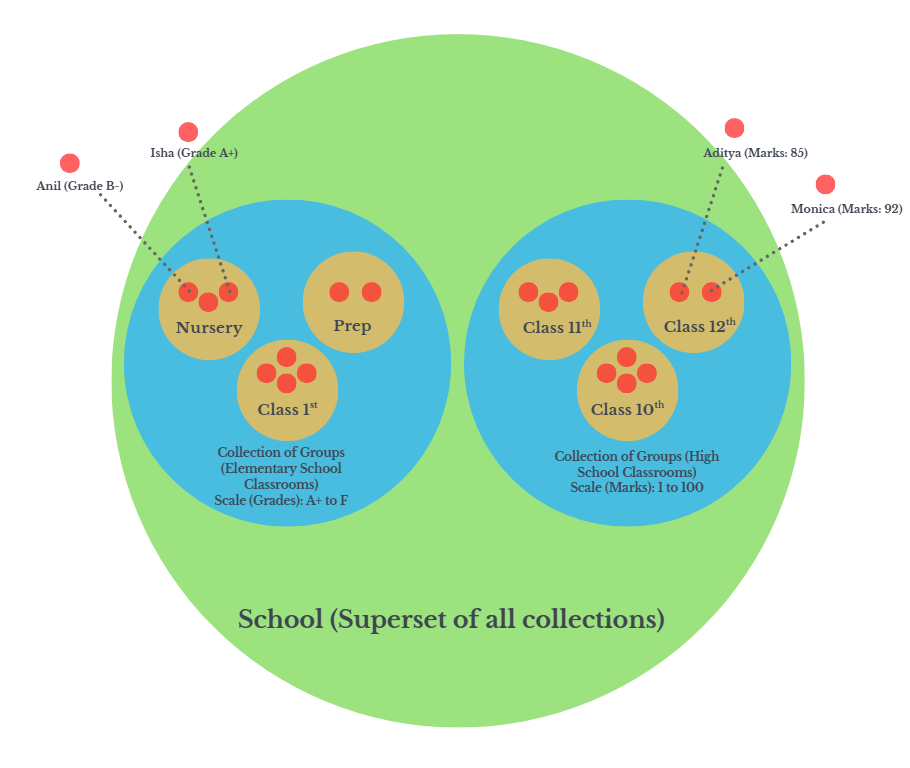
\includegraphics [scale=0.5]{superset_collection.png}
    \caption{Superset Collection of Elementary Grade Groups and High School Groups}
    \label{fig:superset-collection}
\end{figure}

\subsection{Terminologies and Associated Ideas}
The following terms are used throughout this paper:
\begin{definition}
	\textbf{Collection} consists of groups having the same scale of measure for performance.
\end{definition}
\begin{definition}
	\textbf{Group} consists of items, with each item has a rank and its associated value on the scale of measure.
\end{definition}
\begin{definition}
	\textbf{Performance Measure} is a singular value for the performance of a group on a scale indicating worst to best.
\end{definition}

The inspiration for the formula came from the idea from \cite{mann1947test}, which uses median to calculate p-value significance. While the idea draws inspiration from their work, but applied in the context of assessing multiple group performance comparison having unequal elements, and expanded to create a standardize scale with cross-collection interpretability.

These well-known concepts have been used to derive the formulae:
\begin{enumerate}[i]
\item Median Comparison in two groups \ldash Mann–Whitney U Test, \cite{mann1947test}
\item Multiple Group Median Comparison \ldash Kruskal-Wallis H test, \cite{kruskal1952use}
\item Ranked-Based Ordering \ldash Spearman’s Rank Correlation, \cite{spearman1904proof}
\item Ranked-Sum \ldash Wilcoxon Signed-Rank Test, \cite{wilcoxon1945individual}
\item Weight Bias Adjustment \ldash General Bias Correction via Inverse Weighting, \cite{gelman2007survey}
\item Min–Max Normalization \ldash Standard Mathematical Preprocessing, \cite{han2011data}
\end{enumerate}
The novelty is in putting these combination of ideas together, to the concept of Group Performance Analysis and distilling it into a one simple formula called Normalized Performance Measure.

\subsection{Normalized Performance Measure Formulae} 
The discovered formulae to assess performance measure, and is defined as:

\begin{theorem}\label{thm:normalized-performance-measure}
	\textbf{Normalized Performance Measure}, is a performance indicator of a group, in the range of [0,1], indicating a universal scale, from least performance to best, while compensating for the unequalness in the number of elements in a group.
	\begin{equation}
		\boxed{
			\mathbf{
				P_i = \frac{-n_i +  \sum\limits_{j=1}^{n_i} r_j}{n_i \cdot (N - 1)}}
		}
	\label{eq:normalized-performance-measure}	
	\end{equation}
where,
	\begin{itemize}
		\item[] \textbf{$P_i$}: Normalized Performance Measure value of the $i^{th}$ group in the range of [0, 1]
		\item[] \textbf{$\sum r_j$}: Sum of ranks\footnote{{\textbf{Ranks}: Sequential ranks assigned to items within and across groups. Tied ranks are averaged out. Note ranks are in ascending order of performance i.e. rank 1 and rank $N^{th}$ are the worst and best performer respectively. This is done to keep symmetry with usage of ranks in other statistics methods such as \cite{mann1947test} etc.}} for group $i$.
		\item[] \textbf{$n_i$}: number of elements within the $i^{th}$ group
		\item[] \textbf{$k$}: number of groups in the collection
		\item[] \textbf{$N$}: Total number of elements across all group combined
		\begin{align*}
			\text{N} = \sum\limits_i^k n_i
		\end{align*}
	\end{itemize}
\end{theorem}

This formula is the conclusion of the research paper for distilling the Group Performance Analysis to a simplified formulae for practical application.

\begin{pot}[\ref{thm:normalized-performance-measure}]
	Normalizing the Non-normalized Performance Measure, $p_i^{(non\text{-}normalized)}$\footnote{the definition of \autoref{thm:non-normalized-performance-measure}}, into a standardized scale with bounds [0,1], making it independent of the minima and maxima of that particular collection.
\end{pot}

\subsection{Applications}
This is a list of Applications\footnote{There could be applications outside the scope of this paper. But, when designing the formula these listed applications were being considered.} scenario, the formula was designed for:
\begin{itemize}
	\item \textbf{Psychology}: In Psychology, we have a big arsenal of therapy techniques, all having their own benefits. If, mutually exclusive groups, each group taking a particular therapy, needs to be analyzed which group performed better, and the group sizes are unequal. Then, Performance Measure Formula can be applied.
	\item \textbf{Medical}: Similarly, sometimes Drugs treating the same illness, are compared to each other. Even, prototypes of the same Drugs are compared amongst themselves when in research phase. In these scenarios, even if, the sample size of each drug is unequal, Normalized Performance Measure Formulae can be applied for comparison.
    \item \textbf{Educational}: Awarding Best Class Performance, in a school, when classes have unequal number of students, and even different grading scales.
    \item \textbf{Organizational}: To identify best-performing team in the organization, and least-performing, for restructuring and guidance purposes, when number of person per team are unequal, and performance scale at various sector of an organization is different.
   \item \textbf{Business}: Often businesses have economy segment and luxury segment for services and products. Often, just price is not an enough indicator what segment of products fared better. If, a ranking is created, on customer feedback, return on investment, maintenance-cost, advertisement, market reach etc. Then, this formula can be used to find the dominant product/services of their business, when there is unequal sale of each product/services sold.
\end{itemize}

\subsection{Scope of the Research Paper}
The paper will present the theoretical foundation and mathematical derivation of the proposed measure, accompanied by logical justifications and where applicable visual intuitions to enhance conceptual understanding. The range of the normalized performance measure, bounded between 0 and 1, will be proven as well. Furthermore, the performance measure formula would be validated mathematical analysis, numerical simulations, and cross-validation against established statistical methods. A detailed example will also be provided to demonstrate the practical applicability and interpretability of the method.

\section{Non-normalized Performance Measure}

\newdefinition{nonNormalizedPerformanceMeasure}{Definition}
\begin{theorem} \label{thm:non-normalized-performance-measure}
	\textbf{Non-normalized Performance Measure} is a performance indicator for a group that compensates for unequal group sizes by introducing a weighted bias. The measure operates on a local scale defined by the collection-specific minima and maxima i.e. least to best performance, and is dependent on the number of groups and their respective sizes.
	
	\begin{equation}
		p_i^{(non\text{-}normalized)} = w_i \cdot \frac{\sum r_j}{ S_{UDH} }
		\label{eq:non-normalized}
	\end{equation}
	
	where, minima and maxima of the collection is given by:
	\begin{align*}
	p_i^{(min, \, non\text{-}normalized)} = 
	\begin{cases}
			\frac{8}{k(3N + 2)}
			 & \text{if, } N \text{ is even} \\
			\frac{8N}{k (N+1)(3N+1)}, & \text{if, } N \text{ is odd}
	\end{cases}
	\end{align*}
	
	\begin{align*}
		p_i^{(max, \, non\text{-}normalized)} = 
		\begin{cases}
			\frac{8N}{k(3N + 2)}, & \text{i,f } N \text{ is even} \\
			\frac{8N^2}{k (N+1)(3N+1)}, & \text{if, } N \text{ is odd}
		\end{cases}
	\end{align*}
	
	Sum of Upper Dominant Half is given by:
	\begin{align*}
		S_{UDH} = \frac{N(N+1)}{2} - \frac{a(a+1)}{2}, \quad \text{where } a = \lfloor N/2 \rfloor
	\end{align*}
	
	and the weight bias is given by:
	\begin{align*}
		w_i = \frac{N}{k n_i}
	\end{align*}

	
\end{theorem}

\begin{pot}[\ref{thm:non-normalized-performance-measure}]
	The ratio of ranked sum of the particular group and sum of upper dominant half will indicate a local (biased) performance measure, and subsequently made unbiased for unequal group sizes by introducing a weight bias.
\end{pot}

If you see, the \autoref{fig:dominance_Understanding}, its intuitively easy to understand that Group B performance is more dominant, than Group A, simply because Group B occupy the higher ranks, and Group A lower.
\begin{figure}
    \caption{Visual intuition of the Performance Measure, Performance: Group B > Group A}
    \centering
    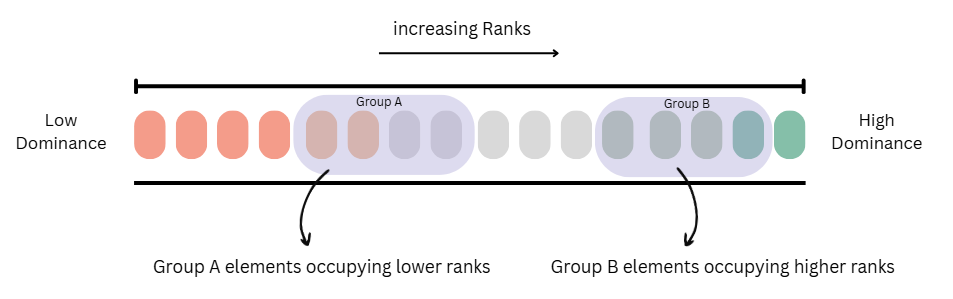
\includegraphics[scale=0.65]{dominance-intuition.png}
    \label{fig:dominance_Understanding}
\end{figure}

This non-normalized performance measure would be used later in the paper to derive the normalized version of the formula. Thus, non-normalized performance measure, $p_i^{(non\text{-}normalized)}$\footnote{
	can also be written as, $p_i^{(non\text{-}normalized)} = w_i \cdot p_i^{(biased)} \text{, where, } p_i^{(biased)}= \frac{\sum r_j}{ S_{UDH} }$ discussed in \autoref{thm:non-normalized-biased-performance-measure} of the research paper}, derivation would be discussed first.

\subsection{Derivation of Non-normalized Performance Measure}

From, the understanding we gain from \autoref{fig:dominance_Understanding}, we can easily, ascertain the local dominance, if we divide the scale into two halves of lower ranks half, and upper rank half. So, the group with ranks in the upper half would have a more prominent or dominant performance. So, we need to figure out what's the ranks of the upper dominant half is.

\subsubsection{Sum of Upper Dominant Half}
\begin{theorem} \label{thm:sum-upper-dominant-half}
	\textbf{Sum of upper dominant half} is rank summation of the upper half of the sequential ranks of natural numbers.
		
	\begin{equation}
		S_{UDH} = \frac{N(N + 1)}{2} - \frac{a(a+1)}{2}
		\label{eq:SUDH}
	\end{equation}
	
	where,
	 \( a = \lfloor \frac{N}{2} \rfloor \) represents the size of the non-dominant half (lower half).
	 
	also can be written in the form of:
	\begin{align*}
	 S_{UDH} =
	 \begin{cases}
	 	\frac{N(3N + 2)}{8},
	 	& \text{if, } N \text{ is even} \\
	 	\frac{(N + 1)(3N + 1)}{8}, & \text{if, } N \text{ is odd}
	 \end{cases}
	\end{align*}
\end{theorem}

\begin{pot}[\ref{thm:sum-upper-dominant-half}]
	Apply Sum of Arithmetic Progression Formula to upper half of the sequential series for Natural Numbers.
\end{pot}
 
Purpose of the Upper Dominant Half (UDH) is to provide benchmark for performance analysis in rank-based comparisons.

Derivation of $S_{UDH}$:
\begin{enumerate}[i.]
\item{
	Total Rank Sum for a dataset of natural numbers with N items, the total rank sum is
	\begin{align*}
		S = 1 + 2 + 3 + \ldots + N
	\end{align*}
	Using the formula for the sum of the first \( N \) integers:
	\begin{align*}
		S = \frac{N(N + 1)}{2}
	\end{align*}
}

\item{
	Split the Dataset into Halves
	\begin{itemize}
	  \item \( a = \lfloor \frac{N}{2} \rfloor \) represents the size of the non-dominant half (lower half).
	  \item The dominant upper half includes the rank from \( a + 1 \) to \(N^{th}\) rank items.
	\end{itemize}
}

\item{Rank Sum of non-dominant Half (lower half) consists of the smallest \( a \) ranks. Its rank sum is:
	\begin{align*}
		S_{lower} = 1 + 2 + \ldots + a
	\end{align*}
	Using the formula for sum of integers:
	\begin{align*}
		S_{lower} = \frac{a(a+1)}{2}
	\end{align*}
}

\item{Rank Sum of Dominant Half (Upper Half)
	The Upper Dominant Half is calculated by subtracting the rank sum of the lower half from the total rank sum:
	\begin{align*}
	S_{UDH} = S - S_{lower}
	\end{align*}
	Substituting the formulas:
	\begin{align*}
	S_{UDH} = \frac{N(N + 1)}{2} - \frac{a(a+1)}{2}
	\end{align*}
}

\item{Final Formula for Sum of Upper Dominant Half:}
\begin{align*}
S_{UDH} = \frac{N(N + 1)}{2} - \frac{a(a+1)}{2}
\label{eq:SUDH}
\end{align*}

where,
\begin{itemize}
  \item[] \( N \): Total number of items.
  \item[] \( a \): Size of the lower \textbf{dominant half}, calculated as the floor of half of the net total number of items across the collection, so as to be inclusive of both odd and even count of N items:
  \begin{align*}
  a = \lfloor \frac{N}{2} \rfloor
  \end{align*}
\end{itemize}
\end{enumerate}

\begin{enumerate}[\textit{Scenario:}] 
	\item \textbf{N is even} i.e net total number of items across all groups is even then it's safe to assume that:
	\begin{align*}
		a = \frac{N}{2}
	\end{align*}
	Thus, the lower and upper halves would be explicitly:
	\[
	\left[1, \frac{N}{2}\right] \quad \text{and} \quad \left[\frac{N}{2}+1, N\right]
	\]
	Simplifying $S_{UDH}$ by applying the Sum of Arithmetic Progression formulae for the upper half:
	\begin{align*}
		S_{UDH} = \frac{N(3N + 2)}{8}
	\end{align*}
	When N is even, the \autoref{thm:sum-upper-dominant-half} is derived.
	
	\item \textbf{N is odd} where $N^{(min)} = 3$, because there has to be minimum of two groups, therefore,  its safe to assume that,
	\begin{align*}
		a = \frac{N-1}{2}
	\end{align*}
	
	Thus, the lower and upper halves would be explicitly:
	\[
	\left[1, \frac{N-1}{2}\right] \quad \text{and} \quad \left[\frac{N+1}{2}, N\right]
	\]
	
	Applying the sum of arithmetic progression formula to upper half, we get:
	\begin{align*}
		S_{UDH} = \frac{(N+1)(3N+1)}{8}
	\end{align*}
	Hence, when N is odd, \autoref{thm:sum-upper-dominant-half} is derived.
\end{enumerate}

\subsubsection{Non-normalized Performance Formulae (Biased)}


\begin{theorem}\label{thm:non-normalized-biased-performance-measure}
	Non-normalized Performance Formuale (Biased), is the unweighted performance indicator of the group, inconsiderate to group sizes, and therefore biased.
\begin{equation}
    p_i^{(biased)} = \frac{\sum r_j}{ S_{UDH} }
 \label{eq:p-biased}
\end{equation}
where,
\begin{itemize}
    \item[] \textbf{$\sum r_j$}: Sum of ranks for group $i$.
    \item[] \textbf{$S_{UDH}$}: Sum of Upper Dominant Half
\end{itemize}
\end{theorem}

\begin{pot}[\ref{thm:non-normalized-biased-performance-measure}]
	The ratio of ranked sum of the particular group and sum of upper dominant half will indicate a local (biased) performance measure, which is benchmark against upper dominant half ranks in the collection. 
\end{pot}

As we have aleady derived the Sum of Upper Dominant half, $S_{UDH}$, in \autoref{thm:sum-upper-dominant-half}. Substituting the value, completes the definition of \autoref{thm:non-normalized-biased-performance-measure}.

As, the formula doesn't take into account weight bias. A high number of items can still occupy lower ranks, but in account of total items in group being large, its ranked sum also gives a higher value. That's why weight bias was added to adjust this non-normalized performance measure.

\subsubsection{Weight Bias}
\begin{theorem}\label{thm:weight-bias}
	\textbf{Weight Bias}
	 for each group is defined as the fractional adjustment required for that group’s size to reach the ideal equal group size, where the ideal is the mean of all group sizes in the collection.
	\begin{equation}
		w_i = \frac{N}{kn_i}
		\label{eq:weight-bias}
	\end{equation}
	
	where:
	\begin{itemize}
		\item[] $w_i$: Weight bias for group $i$.
		\item[] $n_i$: Number of items in group $i$.
		\item[] $N$: Total number of items.
		\item[] $k$: Number of groups.
	\end{itemize}
	also can be written in the form of,
	\begin{align*}
		w_i = \frac{\bar{n}}{n_i}
	\end{align*}
	where:
	\begin{itemize}
		\item[] $\bar{n}$: Mean of group sizes in the collection
		\item[] $n_i$: Number of items in group $i$.
	\end{itemize}
\end{theorem}

In other words, Weight Bias is the fractional adjustment multiplicative factor applied to the \textbf{Biased Performance Measure}\footnote{also named Non-Normalized Performance Measure (Biased). See the definition of \autoref{thm:non-normalized-biased-performance-measure}} to obtain the unbiased \textbf{Non-normalized Performance Measure}\footnote{See definition of \autoref{thm:non-normalized-performance-measure}}. This compensates for unequal group sizes in the collection.

\begin{pot}[\ref{thm:weight-bias}]
	 The weight bias is visualized as multiplicative correction factor\footnote{similar in spirit to how a percentage gain/loss is applied in economics}.
\end{pot}

The items expected in each group (ideal size), can be written as mean of the group sizes:
\[
\bar{n} = \frac{N}{k}
\]
The fractional change needed to reach \(\bar{n}\) from \(n_i\) is:
\[
\text{Fractional change} = \frac{\bar{n} - n_i}{n_i}
\]

To derive the weight bias ($w_i$), observe that when all groups have equal sizes, no adjustment is needed (i.e $w_i = 1$, as $n_i = \bar{n}$). That means all the groups have the same number of elements in them. 

But, in scenarios of unequal group sizes multiplicative correction is applied:
\[
w_i = 1 + \frac{\bar{n} - n_i}{n_i} = \frac{\bar{n}}{n_i} = \frac{N}{k n_i}
\]

Hence, \autoref{thm:weight-bias} derived.

\subsubsection{Final Formula for unbiased (but non\text{-}normalized) Performance Measure}

As mentioned earlier, biased performance measure is made unbiased by multiplying the adjustment factor (weight bias). Therefore, from \autoref{thm:non-normalized-biased-performance-measure} and \autoref{thm:weight-bias}, we can write:

\begin{align*}
	p_i^{(non\text{-}normalized)} = w_i * p^{(biased)}
\end{align*}


Substituting their corresponding values, we derived the non-normalized performance measure\footnote{In this research paper, $p_i^{(non\text{-}normalized)}$ = $p_i^{(unbiased)}$ are same, but for standardization sake, we will use $p_i^{(non\text{-}normalized)}$ moving forward.}, as stated in the beginning of the section, in \autoref{thm:non-normalized-performance-measure}:
\begin{align*}
    p_i^{(non\text{-}normalized)} = \frac{N}{k n_i} \cdot \frac{\sum r_j}{ S_{UDH} }
\label{p-non-normalized}
\end{align*}

\subsection{Minima and Maxima of Non-normalized Performance Measure}
As the \autoref{thm:non-normalized-performance-measure} i.e. Non-normalized performance measure, is not normalized, so it has a collection specific minima and maxima. In this following section we will derive the range. And later use it to normalize the performance measure to derive the final formula.
\subsubsection{Minima of Non-normalized Performance Measure}
\begin{theorem}\label{thm:non-normalized-minima}
	\textbf{Minima for Non-normalized Performance Measure} is the lowest indicator of performance measure for that collection.
	\begin{equation}
		p_i^{(min, \, non\text{-}normalized)} =
		\begin{cases}
			\frac{8}{k(3N + 2)}, & \text{if, } N \text{ is even} \\
			\frac{8N}{k (N+1)(3N+1)}, & \text{if, } N \text{ is odd}
		\end{cases}
	\end{equation}
\end{theorem}

\begin{pot}[\ref{thm:non-normalized-minima}]
	Minimizing \autoref{thm:non-normalized-performance-measure} i.e \textbf{Non-normalized Performance Measure} which in turn dependent on minimizing $\frac{\sum r_j}{n_i}$.
\end{pot}
\begin{enumerate}[\textit{Scenario:}] 
	\item \textbf{N is even} i.e  net total number of items across all groups is even. So, we already know the sum of upper dominant half when n is even from \autoref{thm:sum-upper-dominant-half}. Recapitulating:
	\begin{align*}
		S_{UDH} = \frac{N(3N + 2)}{8}
	\end{align*}
	We aim to minimize the non-normalized measure $p_i^{(non\text{-}normalized)}$ defined as:
	\begin{align*}
		p_i^{(non\text{-}normalized)} = w_i \cdot \frac{\sum r_j}{ S_{UDH} }
	\end{align*}
	Substituting $S_{UDH}$ (from \autoref{thm:sum-upper-dominant-half}) and $w_i$ (from \autoref{thm:weight-bias}) in above, we get:
	\begin{align*}
		p_i^{(non\text{-}normalized)} = \frac{8}{k(3N + 2)}\cdot \frac{\sum r_j}{n_i}
		\label{eq:simplified-even-non-normalized}
	\end{align*}
	As, 
	\begin{align*}
		\frac{8}{k(3N + 2)} = Constant
	\end{align*}
	Then it follows that, minima depends on $\frac{\sum r_j}{n_i}$. And, for this to be low, $\sum r_j$ should be low. That means $r_j$ have to occupy the lowest ranks such as 1, 2, 3,... so on. We can rewrite $\frac{\sum r_j}{n_i}$ in this format below:
	\begin{align*}
		\frac{\sum r_j}{n_i} = \frac{\frac{n_i}{2}(1+n_i)}{n_i} = \frac{1}{2} \cdot n_i + \frac{1}{2}
	\end{align*}
	As this is a linearly increasing line equation with a positive slope ($y = mx + C$), minima of $\frac{\sum r_j}{n_i}$ occurs when $n_i = 1$, as $n_i$ is a natural number and can't be zero or negative, hence, substituting $n_i = 1$, we get, $\frac{\sum r_j}{n_i} = \frac{1}{2} + \frac{1}{2} = 1$, hence  $\frac{\sum r_j}{n_i} = 1 $
	Therefore when N is even, minima of Non-normalized measure is:
	\begin{align*}
		p_i^{(min, \, non\text{-}normalized)} = \frac{8}{k(3N + 2)}
	\end{align*}
		Hence, when N is even, we derived the minima in \autoref{thm:non-normalized-minima}
	\item \textbf{N is odd}, we already know the sum of upper dominant half \begin{align*}
		S_{UDH} = \frac{(N+1)(3N+1)}{8}
	\end{align*}
	Substituting $S_{UDH}$ (from \autoref{thm:sum-upper-dominant-half}) and $w_i$ (from \autoref{thm:weight-bias}) in \autoref{thm:non-normalized-performance-measure}, 
	we get:
	\begin{align*}
		p_i^{(non\text{-}normalized)} = \frac{8N}{k(N+1)(3N+1)} \cdot \frac{\sum r_j}{n_i}
	\end{align*}
	We have alredy established that $\frac{\sum r_j}{n_i} = 1$,
	if we need to minimize the non-normalized performance measure,  we get:
	\begin{align*}
		p_i^{(min, \, non\text{-}normalized)} = \frac{8N}{k (N+1)(3N+1)}
	\end{align*}
	Hence, when N is odd, we derived the minima in \autoref{thm:non-normalized-minima}
\end{enumerate}

\subsubsection{Maxima of Non-normalized Performance Measure}
\begin{theorem}\label{thm:non-normalized-maxima}
	\textbf{Maxima for Non-normalized Performance Measure} is the highest indicator of performance measure for that collection.
	\begin{equation}
		p_i^{(max, \, non\text{-}normalized)} =
		\begin{cases}
			\frac{8N}{k(3N + 2)}, & \text{if, } N \text{ is even} \\
			\frac{8N^2}{k (N+1)(3N+1)}, & \text{if, } N \text{ is odd}
		\end{cases}
	\end{equation}
\end{theorem}

\begin{pot}[\ref{thm:non-normalized-maxima}]
	Maximizing \autoref{thm:non-normalized-performance-measure} i.e \textbf{Non-normalized Performance Measure} which in turn dependent on maximizing $\frac{\sum r_j}{n_i}$.
\end{pot}
\begin{enumerate}[\textit{Scenario:}] 
	\item \textbf{N is even}, Similar in how we derived the minima, we need to maximize the non-normalize performance measure:
	\begin{align*}
		p_i^{(non\text{-}normalized)} = \frac{8}{k(3N + 2)}\cdot \frac{\sum r_j}{n_i}
	\end{align*}
	As we already know, 
	\begin{align*}
		\frac{8}{k(3N + 2)} = Constant
	\end{align*}
	Maxima depends on $\frac{\sum r_j}{n_i}$, which needs to be maximized. Therefore, $r_j$ will contain higher ranks, such as $N, N-1, N-2,... ,k$. So, the lowest rank in this arithmetic series can contain is k. Because, there are k groups, that means, each will have at least one element, occupying the lowest ranks, to maximize $\frac{\sum r_j}{n_i}$. That means, first group will contain rank 1, second group will contain rank 2, so on..., and the $k^{th}$ group will have the rest of the elements from rank $k^{th}$ to $N^{th}$ element which we are trying to maximize. Then $\sum r_j$, as sum of the arithmetic series  $N, N-1, N-2,... ,k$ can be simplified to:
	\begin{align*}
		\sum r_j = \frac{(N-k+1)(N+k)}{2}
	\end{align*}
	As, $n_i$ are the number of elements in the group which is equal to $N-k+1$, then simplifying $\frac{\sum r_j}{n_i}$, by substituting their corresponding values:
	\begin{align*}
		\frac{\sum r_j}{n_i} = \frac{N+k}{2}
	\end{align*}
	Now to maximize, we can substitute k with N, as k are number of groups, and the max number of groups would be equal to total number of items in the collection, where each group has just one element.
	hence maximum value comes out to be:
	\begin{align*}
		\frac{\sum r_j}{n_i} = N
	\end{align*}
	
	Therefore maxima of Non-normalized Measure is:
	\begin{align*}
		p_i^{(max, \, non\text{-}normalized)} = \frac{8N}{k(3N + 2)}
	\end{align*}
	Hence, when N is even, \autoref{thm:non-normalized-maxima} derived.
	\item \textbf{N is odd}, then we already know sum of upper dominant half for it from \autoref{thm:sum-upper-dominant-half}:
	\begin{align*}
		S_{UDH} = \frac{(N+1)(3N+1)}{8}
	\end{align*}
	
	Substituting $S_{UDH}$ (from \autoref{thm:sum-upper-dominant-half}) and $w_i$ (from \autoref{thm:weight-bias}) in \autoref{thm:non-normalized-performance-measure}, 
	we get:
	
	\begin{align*}
		p_i^{(non\text{-}normalized)} = \frac{8N}{k(N+1)(3N+1)} \cdot \frac{\sum r_j}{n_i}
	\end{align*}
	As we already established, that to maximize, we need to equate $\frac{\sum r_j}{n_i} = N$.
	Therefore,
	\begin{align*}
		p_i^{(max, \, non\text{-}normalized)} = \frac{8N^2}{k(N+1)(3N+1)}
	\end{align*}
	Hence, when N is odd, \autoref{thm:non-normalized-maxima} derived.
\end{enumerate}

\section{Normalized Performance Measure}

The unbiased and non-normalized formulae, is needed to be normalized, for to satisfy these following criteria:
\begin{itemize}
	\item Explicitly provides a meaningful zero baseline for dominance measures.
	\item Performance scores become standardized, allowing direct comparisons across multiple studies or scenarios
\end{itemize}
Given by:
\begin{align*}
	\boxed{
		\mathbf{
			P_i = \frac{-n_i +  \sum\limits_{j=1}^{n_i} r_j}{n_i \cdot (N - 1)}}
	}
\end{align*}
This formulae is the conclusion of whole paper, which is named Normalized Performance Measure defined in the begining of paper in \autoref{thm:normalized-performance-measure}

\subsection{Derivation of Normalized Performance Measure}

So, now to normalize the \textbf{Non-normalize Performance Measure}, we will apply the formula below:
\begin{align*}
	P_i = \frac{p_i^{(non\text{-}normalized)} - p_i^{(min, \, non\text{-}normalized)}}{p_i^{(max, \, non\text{-}normalized)} - p_i^{(min, \, non\text{-}normalized)}}
	\label{eq:normalized-simpler}
\end{align*}

Now substituting their corresponding values, from \autoref{thm:non-normalized-performance-measure}, \autoref{thm:non-normalized-minima} and \autoref{thm:non-normalized-maxima}, and simplifying we get the final form of Normalized Performance Measure:
\begin{align*}
	\boxed{
		\mathbf{
			P_i = \frac{-n_i +  \sum\limits_{j=1}^{n_i} r_j}{n_i \cdot (N - 1)}}
	}
\end{align*}
\begin{itemize}
	\item[] \textbf{$P_i$}: Normalized Performance Measure value of the $i^{th}$ group in the range of [0, 1]
	\item[] \textbf{$\sum r_j$}: Sum of ranks for group $i$.
	\item[] \textbf{$n_i$}: number of elements within the $i^{th}$ group
	\item[] \textbf{$N$}: Total number of elements across all group combined.
\end{itemize}

\subsection{Range of Normalized Performance Measure}
Minima of Normalized Performance Measure, $P_i = 0$. In other words, is the least dominant performance in the entire collection. This happens when a group contains one element with Rank 1. Mathematically, $p_i^{(non\text{-}normalized)} =  p_i^{(min, \, non\text{-}normalized)}$, and normalizing the non-performance measure, we will get:
\begin{equation}
	P_i^{(min)} = \frac{p_i^{(min, \, non\text{-}normalized)} - p_i^{(min, \, non\text{-}normalized)}}{p_i^{(max, \, non\text{-}normalized)} - p_i^{(min, \, non\text{-}normalized)}} = 0
\end{equation}

Similarly,
Maxima of $P_i^{(max)} = 1$. In other words, is the most dominant performance in the entire collection. This happens when a group contains one element with Rank $N^{th}$, the highest ranked element possible. Mathematically, $p_i^{(non\text{-}normalized)} =  p_i^{(max, \, non\text{-}normalized)}$, and normalizing the non-performance measure, we will get:
\begin{equation}
	P_i^{(max)} = \frac{p_i^{(max, \, non\text{-}normalized)} - p_i^{(min, \, non\text{-}normalized)}}{p_i^{(max, \, non\text{-}normalized)} - p_i^{(min, \, non\text{-}normalized)}} = 1
\end{equation}

Therefore, the range of normalized performance measure is [0,1]


\section{Validation}
A theoretical research is only holistic if, validated mathematically\footnote{done via SymPy Library in Python/Jupyter Notebook}, numerically\footnote{done via Python OOPs} and cross-validated via existing established methods\footnote{done via SciPy's Statistics Library}. So, in this section this is what we intend to do so.

All mathematical and numerical validation scripts, as well as the full manuscript source, are available in the GitHub repository \cite{silentkarmi2025normalized}. See the repository's folder structure and README for details on specific files and validation types.

\subsection{Numerical Cross-validation with existing Statistical Methods}
Normalized Performance Measure indicates a value which tells us the group performance dominance, if it's closer to 1, then that group performed exceptionally well. And, if its closer to 0, then it was a dismissal performance. If, we can establish a relationship between p-Value and Normalized Performance Measure. Then this result can be used to cross-validate Normalized Performance Measure.

\subsubsection{Relationship with p-value}
With Normalized Performance Measure, there is a intuitive relationship with the significane value. For instance along with Control Group, if we need to know what experimental group performed better or worse. This can be achieved by following the approach discussed.

Apply, \cite{kruskal1952use} H Test. Then, using the 'H' characteristic, the significance value can be calculated. If p-value $\le$ 0.05, then we can reject the null hypothesis. This means that one or more experimental groups have shown deviation. Now, we can use a post-hoc \cite{dunnett1955multiple} test to see, if any experimental group has shown deviation. Now, one question is still left unanswered. Now, is this deviation negative or positive i.e. experimental group performed well or worse than the control group, (assuming we have performed two-tailed test for p-value). Now, we can use Normalized Performance Measure to understand, if these experimental groups performed exceptionally well, dismissal, or about the same.
\begin{center}
	\begin{tabular}{|c|c|l|}
		\hline
		\textbf{p-value} & \textbf{Deviation} & \textbf{Normalized Performance Measure} \\
		\hline
		$\leq 0.05$ & Yes & Dismissal = closer to 0 or Exceptional = closer to 1 \\
		\hline
		$> 0.05$ & No & Closer to 0.5 (mid-performing groups) \\
		\hline
	\end{tabular}
	\vspace{2pt}
	\captionof{table}{Interpretation of p-values in relation to deviation and normalized performance}
	\label{table:p-value-relationship}
\end{center}
So, if we are able to show numerically, by taking an example, that the results follow the same results as in summarized in the \autoref{table:p-value-relationship}, then Normalized Performance Measure can be said to be validated.

\subsubsection{Simulated Data Numerical Cross Validation: Medical Drug Performance}
To cross validate the relationship between pValue and Normalized Performance measure, along with a Control Group, we would compare three experimental groups with Drug A, Drug B and Drug C. This simulated data\footnote{fictitious data is being used} is shown in the form of BoxPlot in \autoref{fig:box-plot}, 
\begin{figure}
	\caption{Drugs comparison and showing relationship between Permormance Measure and pValue}
	\centering
	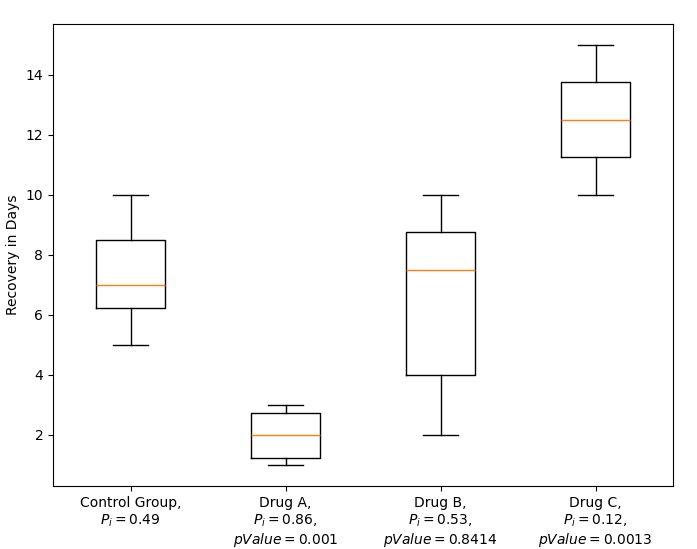
\includegraphics [scale=0.65]{simulation-data-kruskal-dunnett.png}
	\label{fig:box-plot}
\end{figure}
on which we have performed the Kruskal Wallis H Test and Dunnett's Test. And, the results are summarized in the table below:
	

\begin{center}
	\begin{tabular}{lccccc}
		\toprule
		\textbf{Group} &
		\makecell{\textbf{Kruskal-Wallis} \\ \textbf{'H' Test (pValue)}} &
		\makecell{\textbf{Group} \\ \textbf{Deviation (Y/N)}} &
		\makecell{\textbf{Dunnett's} \\ \textbf{Test (pValue)}} &
		\makecell{\textbf{Deviation} \\ \textbf{(Yes/No)}} &
		\makecell{\textbf{Normalized} \\ \textbf{Performance} \\ \textbf{Measure}} \\
		\midrule
		Control &         &     & -      & -    & 0.49 \\
		Drug A  &         &     & 0.001  & Yes  & 0.86 \\
		Drug B  &         &     & 0.8414 & No   & 0.53 \\
		Drug C  & \multirow{-3}{*}{0.00045} & \multirow{-3}{*}{Yes} & 0.0013 & Yes & 0.12 \\
		\bottomrule
	\end{tabular}
	\vspace{5pt}
	\captionof{table}{Group-wise statistical comparison with normalized performance measure. Note: pValue < 0.05 is considered as deviation}
	\label{table:results-simulated-data}
\end{center}

\textbf{Interpretation of Results}:
As seen in  \autoref{fig:box-plot}, visually, it can be seen that Drug A and Drug C show deviation significantly. This is confirmed numerically in \autoref{table:results-simulated-data}. Because Kruskal Wallis 'H' Test results in pValue < 0.05 therefore, we need to reject the null hypothesis that "these Drugs Performance belong to the same distribution as of Control Group". Because, there is a deviation amongst the group. Dunnett's test pValue confirms which group has deviated which is Drug A and Drug C. If, the deviation indicates best or worst performance is indicated by the Normalized Performance Measure validating the relationship in \autoref{table:p-value-relationship}, as Drug A is closer to 1 (Exceptional Performance), Drug C is closer to 0 (Dismissal Performance) and Drug B shows similar performance measure to control group which is closer to 0.5

\subsection{Mathematical Validation: Theoretical Derivation via SymPy Library in Python}
To, validate all manual work, the formula also has been derived through mathematical coding via SymPy library using Python Language (a open source replacement tool for Mathematica), written inside a Jupyter Notebook.

A snippet of the code is hereby attached: \hyperref[code:snippet_odd_performance_measure]{Python (SymPy) Code Snippet}. This snippet simplifies and factorizes to get Normalized Performance Measure (when N is odd)j, acting as a validation for manual mathematical work.

\autoref{fig:output-mathematical-validation} shows the output for the same.
 	
\begin{mintedbox}{python}
	# Python (SymPy) Code Snippet
	display("N is odd then,")
	
	a = (n - 1)/2
	s_udh = n*(n+1)/2 - a*(a+1)/2
	display("S_UDH = ",simplify(s_udh))
	
	p_i = w_i * sigma_r_j / s_udh
	display("p_i_normalized = ", simplify(p_i))
	
	p_i_min = p_i.subs({n_i:1}) # number of elements = 1
	p_i_min = p_i_min.doit()
	p_i_min = p_i_min.subs({r[1]:1}) # containing one element rank = 1
	display("p_i_minima_non-normalized = ",simplify(p_i_min))
	
	p_i_max = p_i.subs({n_i:1}) # number of elements = 1
	p_i_max = p_i_max.doit()
	p_i_max = p_i_max.subs({r[1]:n}) # containing one element rank = Nth
	display("p_i_maxima_non-normalized = ",simplify(p_i_max))
	
	P_i = (p_i - p_i_min)/(p_i_max - p_i_min)
	display("Normalized Performance Measure, P_i = ", factor(simplify(P_i)))
\end{mintedbox}
\label{code:snippet_odd_performance_measure}


\begin{figure}
	\caption{Output: Mathematical Derivation of Normalized Performance Measure via SymPy}
	\centering
	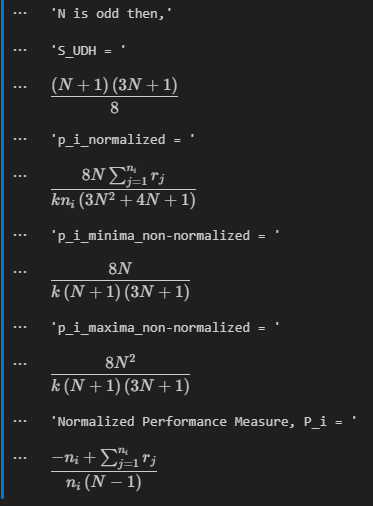
\includegraphics [scale=0.75]{output-mathematical-validation.png}
	\label{fig:output-mathematical-validation}
\end{figure}

\subsection{Numerical Validation: Range of Normalized Performance Measure}
We have mathematically and theoretically have proven the range to [0,1].
Zero means the group has single element with Rank 1 element, lowest performance measure value possible.
And, one means the group has single element with Rank $N^{th}$ element, highest performance measure value possible.
Any combination of elements in the group will be in the range of [0,1].

We have used this simple numerical example to validate the theoretical Maxima and Minima, where value is same as their rank.
\begin{center}
	\begin{tabular}{llcc}
		\toprule
		\textbf{Group} & \textbf{Member Value} & \textbf{Rank} & \textbf{Normalized Performance Measure} \\
		\midrule
		I     & 1   & 1   & 0.0 \\
		\midrule
		\multirow{9}{*}{II} 
		& 2   & 2   & \multirow{9}{*}{0.5} \\
		& 3   & 3   &  \\
		& 4   & 4   &  \\
		& 5   & 5   &  \\
		& 6   & 6   &  \\
		& 7   & 7   &  \\
		& 8   & 8   &  \\
		& 9   & 9   &  \\
		& 10  & 10  &  \\
		\midrule
		III   & 11  & 11  & 1.0 \\
		\bottomrule
	\end{tabular}
	\captionof{table}{Example used for Validation of Range for Normalized Performance Measure}
	\label{table:validation}
\end{center}


This is numerically validated via Python code, by applying the formulae discussed in the research paper, the \hyperref[code:numerical-validation-minima-maxima]{Code Snippet: Numerical Maxima and Minima Validation} is attached below:
\begin{mintedbox}{python}
	def setPerformanceMeasureValue(self):
	"""Calculates the normalized performance value, using the formula
	"""
	ni = self.getElementCount()
	sigma_ri = self.getRankedGroupSum()
	n = self.parent.netTotalItemsInCollection
	k = self.parent.getNumberOfGroups()
	self.performanceMeasureValue = (-ni + sigma_ri)/(ni*(n-1))
\end{mintedbox}
\label{code:numerical-validation-minima-maxima}

See \autoref{fig:output-numerical-validation-minima-maxima}, the output for the \hyperref[code:numerical-validation-minima-maxima]{Code Snippet: Numerical Maxima and Minima Validation}.
\begin{figure}
	\caption{Output: Numerical Validation of Range for Normalized Performance Measure via Python}
	\centering
	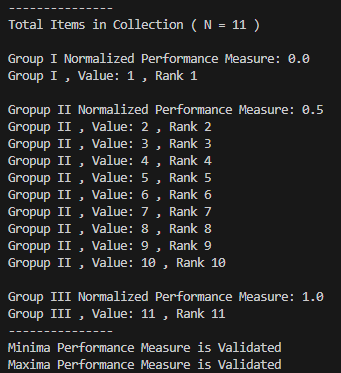
\includegraphics [scale=0.75]{output-validation-minima-maxima.png}
	\label{fig:output-numerical-validation-minima-maxima}
\end{figure}


\section{Detailed Example for Normalized Performance Method Execution}

To explicitly demonstrate the utility and robustness of the Normalized Performance Measure method, we construct a simulated example (not representing real data set) meeting all of the following criteria:

\begin{itemize}
	\item Multiple groups ($k = 4$)
	\item Unequal number of items per group (each group n i.e $n_i >= 3$)
	\item Tied ranks (items's frequency $>=1$)
	\item Total number of participants is odd ($N = 15$)
\end{itemize}
\begin{enumerate}[Step 1.]
	\item Data-set: Each group represents a therapy technique, where participant's give a post-therapy feedback out of 15. Higher scores indicate better performance. Control groups are the participants, who just spent time alone with their thoughts. All the participants are going through a tough life situation of Divorce.\footnote{Fictitious data used for demonstration purposes only and doesn't represent the true effectiveness of the therapy}
	\begin{center}
		\begin{tabular}{|l|l|}
			\hline
			\textbf{Group} & \textbf{Post-Therapy Scores} \\
			\hline
			Control (n = 3) & 6, 12, 12 \\
			CBT (n = 5) & 14, 15, 13, 13, 15 \\
			Mindfulness (n = 4) & 9, 8, 8, 7 \\
			Psychoanalysis (n = 3) & 2, 1, 3 \\
			\hline
		\end{tabular}
		\captionof{table}{Post-therapy improvement scores by group}
	\end{center}
	
	\item Assign Ranks (Handling Ties): Ranks are assigned in ascending order. Tied scores receive the average of their rank positions.
	\begin{center}
		\begin{tabular}{|c|c|c|}
			\hline
			\textbf{Score} & \textbf{Frequency} & \textbf{Assigned Rank} \\
			\hline
			1 & 1 & 1 \\
			2 & 1 & 2 \\
			3 & 1 & 3 \\
			6 & 1 & 4 \\
			7 & 1 & 5 \\
			8 & 2 & 6.5 \\
			9 & 1 & 8 \\
			12 & 2 & 9.5 \\
			13 & 2 & 11.5 \\
			14 & 1 & 13 \\
			15 & 2 & 14.5 \\
			\hline
		\end{tabular}
		\captionof{table}{Assigned ranks (ties averaged)}
	\end{center}
	\item Group-wise Ranked Values:
	\begin{center}
		\begin{tabular}{|l|l|c|c|}
			\hline
			\textbf{Group} & \textbf{Ranks} & $\sum r_j$ & $n_i$ \\
			\hline
			Control & 4, 9.5, 9.5 & 23 & 3 \\
			CBT & 13, 14.5, 11.5, 11.5, 14.5 & 65 & 5 \\
			Mindfulness & 8, 6.5, 6.5, 5 & 26 & 4 \\
			Psychoanalysis & 2, 1, 3 & 6 & 3 \\
			\hline
		\end{tabular}
		\captionof{table}{Group-wise ranks and rank sums}
	\end{center}
	
	\item Apply the Normalized Performance Formula. The normalized performance measure $P_i$ is defined as:
	\[
	P_i = \frac{-n_i + \sum r_j}{n_i (N - 1)}
	\]
	Where $N = 15$ (total items).
	Calculated values for each group:
	\begin{center}
		\begin{tabular}{|l|c|c|c|c|}
			\hline
			\textbf{Group} & $n_i$ & $\sum r_j$ & Formula Result & $P_i$ \\
			\hline
			Control & 3 & 23 & $\frac{-3 + 23}{3 \times 14}$ & 0.476 \\
			CBT & 5 & 65 & $\frac{-5 + 65}{5 \times 14}$ & 0.857 \\
			Mindfulness & 4 & 26 & $\frac{-4 + 26}{4 \times 14}$ & 0.393 \\
			Psychoanalysis & 3 & 6 & $\frac{-3 + 6}{3 \times 14}$ & 0.071 \\
			\hline
		\end{tabular}
		\captionof{table}{Normalized Performance Calculations}
	\end{center}
	
	\item Interpretation of Performance Values
	\begin{itemize}
		\item \textbf{Control}: $P_i = 0.476$ → Baseline for performance
		\item \textbf{CBT}: $P_i = 0.857$ → Exceptional group performance
		\item \textbf{Mindfulness}: $P_i = 0.393$ → Slightly below Control
		\item \textbf{Psychoanalysis}: $P_i = 0.071$ → Dismissal performance
	\end{itemize}
\end{enumerate}
These results are also shown via code: \autoref{fig:box-plot-detailed-example-output}. And they also confirm to the \autoref{table:p-value-relationship} i.e. pValue of CBT and Psychoanalysis <= 0.05, and deviated from the control group, indicating exceptional and dismissal performance respectively.
\begin{figure}
	\caption{Output of the Detailed Example via Python Code:}
	\centering
	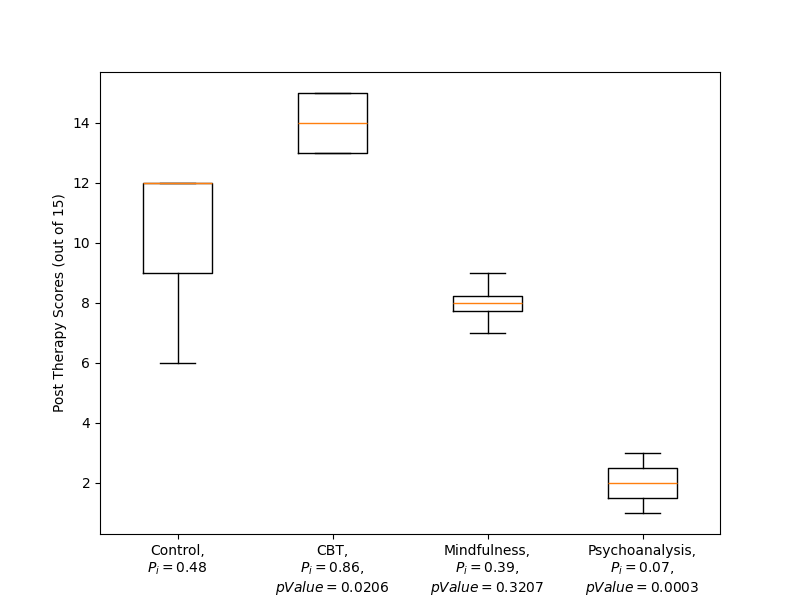
\includegraphics [scale=0.65]{output-detailed-example.png}
	\label{fig:box-plot-detailed-example-output}
\end{figure}
\section{Conclusion}
This work methodically introduced a novel approach to Group Performace Analysis for even unequal group elements, by deriving the Normalized Performance Measure which indicates the performance on a universal scale of range [0, 1] where 0 and 1 denotes the worst and best performance respectively.

\pagebreak
\bibliographystyle{refs-model}
\bibliography{refs}
\appendix
\end{document}